\documentclass[10pt, letterpaper]{article} 

\usepackage[margin=1in]{geometry}
\usepackage{amsfonts, amssymb, amsmath}
\usepackage{tikz,pgfplots}
\usepackage{graphicx}
\usepackage{float}

\def\eq1{y=\dfrac{x}{3x^2+x+1}}

\newcommand{\set}[1] {\setlength\itemsep{#1 em}}

\newcommand\calculator{\tikz{
		\node (c) [inner sep=0pt, draw, fill=black, anchor=south west]{\phantom{N}};
		\begin{scope}[x=(c.south east),y=(c.north west)]    \fill[white] (.1,.7) rectangle (.9,.9);    
		\foreach \x in {.1, .33, .55, .79}{    
		\foreach \y in {.1, .24, .38, .53}{    
		\fill[white] (\x,\y) rectangle +(.11,.07);}} 
		\end{scope} }}
		\def\calcicon#1{\noindent#1 \calculator\ }

\begin{document}
 
\textbf{Critical Thinking Questions}

\begin{figure}[H]
\centering
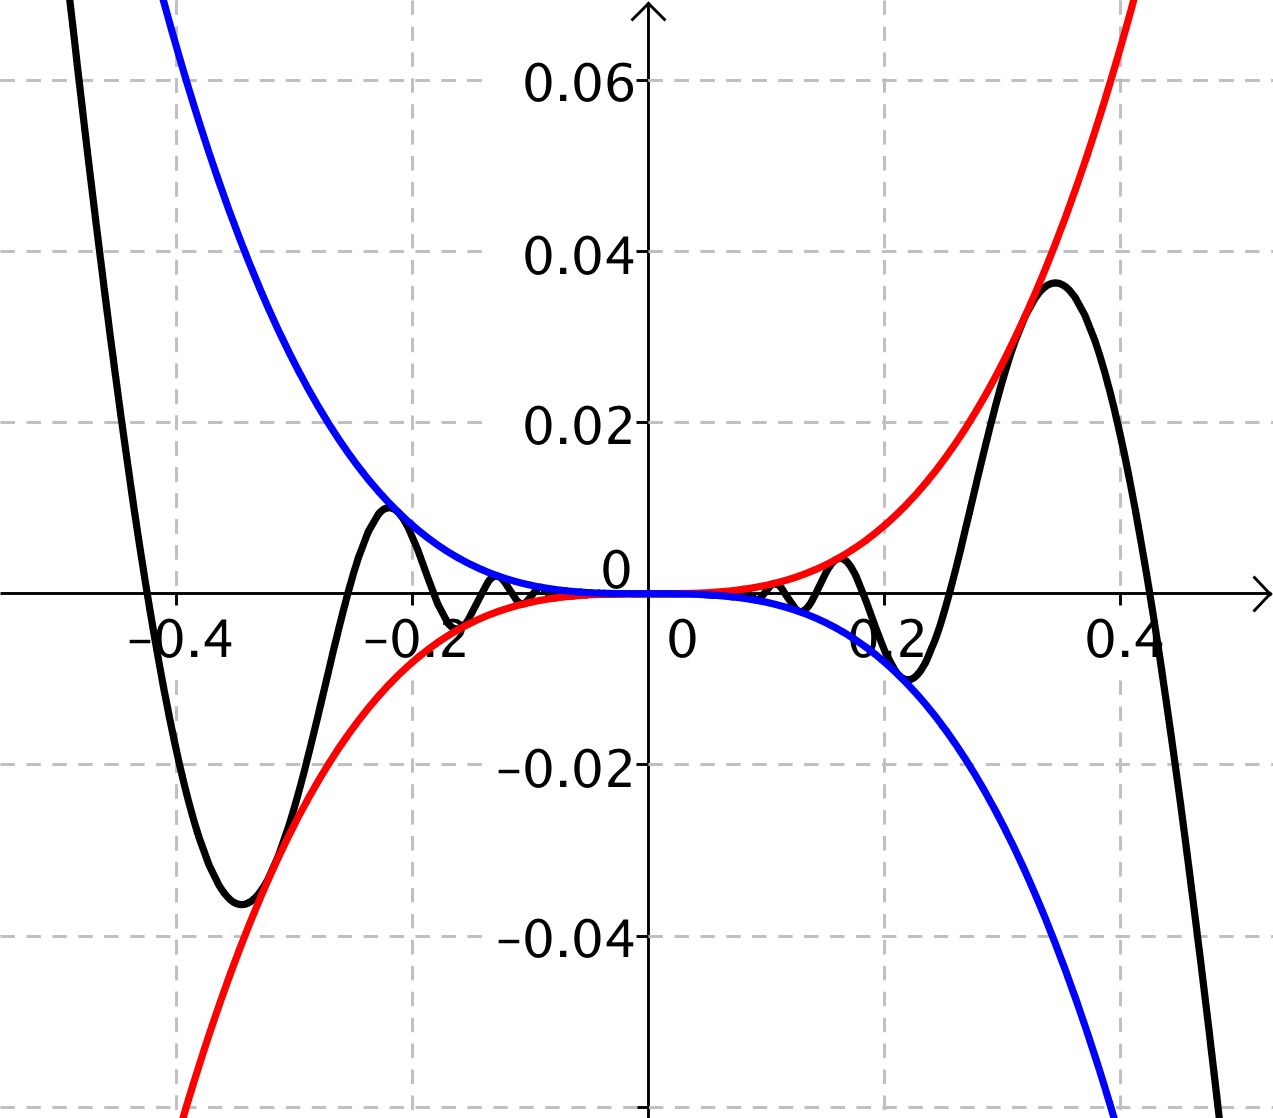
\includegraphics[width=0.4\textwidth]{limit}\\
\caption{The Squeeze Theorem}
\end{figure}


\begin{enumerate}
\set{1.2}
\item \calculator\ Let's examine the function $\eq1$.
\item This is the symbol for the set of all real numbers: $\mathbb{R}$.
\item This is the symbol for the set of integers: $\mathbb{Z}$.
\item This is the symbol for the set of rationals: $\mathbb{Q}$.
\item Is it possible for a sequence to converge to two different numbers? If so, give an example. If not, explain why not.
\item Explain how to use partial sums to determine if a series converges or diverges. Give an example
\item Explain why $\int\limits_{1}^{\infty} f(x)\,dx$ and $\sum\limits_{n=1}^{\infty} a_n$ need not converge to the same value, even if they are both convergent.
\item  In your own words, explain the Alternating Series Remainder Theorem. How is this theorem useful?
\item Explain the difference between absolute and conditional convergence. Give an example of each.
\item The Ratio Test is inconclusive if $\displaystyle{\lim\limits_{n \to \infty} \left| \frac{a_{n+1}}{a_n} \right| =1}$. Give an example of one convergent series and one divergent series for which $\displaystyle{\lim\limits_{n \to \infty} \left| \frac{a_{n+1}}{a_n} \right| =1}$. Explain how you determined your examples.
\end{enumerate}

\end{document}



